% Link to Supplemental Doc:
% https://www.overleaf.com/9488575rxqhnzhzqhgy#/34369899/
% requirements: https://www.nature.com/neuro/pdf/gta.pdf

\documentclass[letterpaper]{article}
%\documentclass[9pt,letterpaper]{article}
\usepackage[top=0.85in,left=1.0in,footskip=0.75in]{geometry}

% Use adjustwidth environment to exceed column width (see example table in text)
\usepackage{changepage}

% Use Unicode characters when possible
\usepackage[utf8x]{inputenc}

% textcomp package and marvosym package for additional characters
\usepackage{textcomp,marvosym}

% fixltx2e package for \textsubscript w
% \usepackage{fixltx2e}

% amsmath and amssymb packages, useful for mathematical formulas and symbols
\usepackage{amsmath,amssymb}

% cite package, to clean up citations in the main text. Do not remove.
\usepackage{cite}
\usepackage{booktabs}

% Use nameref to cite supporting information files (see Supporting Information section for more info)
\usepackage{nameref,hyperref}

% line numbers
\usepackage[right]{lineno}

% ligatures disabled
\usepackage{microtype}
\DisableLigatures[f]{encoding = *, family = * }

% Text layout
\raggedright
\setlength{\parindent}{0.5cm}
\textwidth 6.25in
\textheight 8.75in
\usepackage[aboveskip=1pt,labelfont=bf,labelsep=period,justification=raggedright,singlelinecheck=off]{caption}
\renewcommand{\figurename}{Fig}

\bibliographystyle{plos2015}

% Remove brackets from numbering in List of References
\makeatletter
\renewcommand{\@biblabel}[1]{\quad#1.}
\makeatother

% Leave date blank
\date{}

% Header and Footer with logo
\usepackage{lastpage,fancyhdr,graphicx}
\usepackage{epstopdf}
\pagestyle{myheadings}
\pagestyle{fancy}
\fancyhf{}
\setlength{\headheight}{27.023pt}
\lhead{\sf PNAS Perspectives}
\rfoot{}
\renewcommand{\footrule}{\hrule height 2pt \vspace{2mm}}
\fancyheadoffset[L]{0.0in}
\fancyfootoffset[L]{0.0in}
\lfoot{\sf PNAS Perspectives}


\newcommand{\lorem}{{\bf LOREM}}
\newcommand{\ipsum}{{\bf IPSUM}}

\begin{document}
\vspace*{0.2in}

\begin{flushleft}
{\Large

\textbf{3} Current Address: Ronald Tutor Hall, RTH-404
3710 S. McClintock Ave
\\
\textbf{3}
Current Address: Ronald Tutor Hall, RTH-404
3710 S. McClintock Ave
Los Angeles, CA 90089-2905, USA % change symbol to "\textcurrency a" if more than one current address note
\\
\Yinyang  B.C. and M.S. contributed equally as first authors.

% Use the asterisk to denote corresponding authorship and provide email address in note below.
* valero@usc.edu

\end{flushleft}
% Please keep the abstract below 150 words for NN
\section*{Abstract}


%%%%%%%%%%%%%%%%%%%%%%%%%%%%%%%%%%%%%%%%%%%%%%%%%%%%%%%%%%%%%%%%%%%%%%%%%%%%%%%%%%%%%%%%%%%%%%%%%%%%%%%%

%NATNEURO: "we will continue to ask that authors keep their methods sections to a limit of 2,000 words."

\begin{figure}[htbp]
\centering
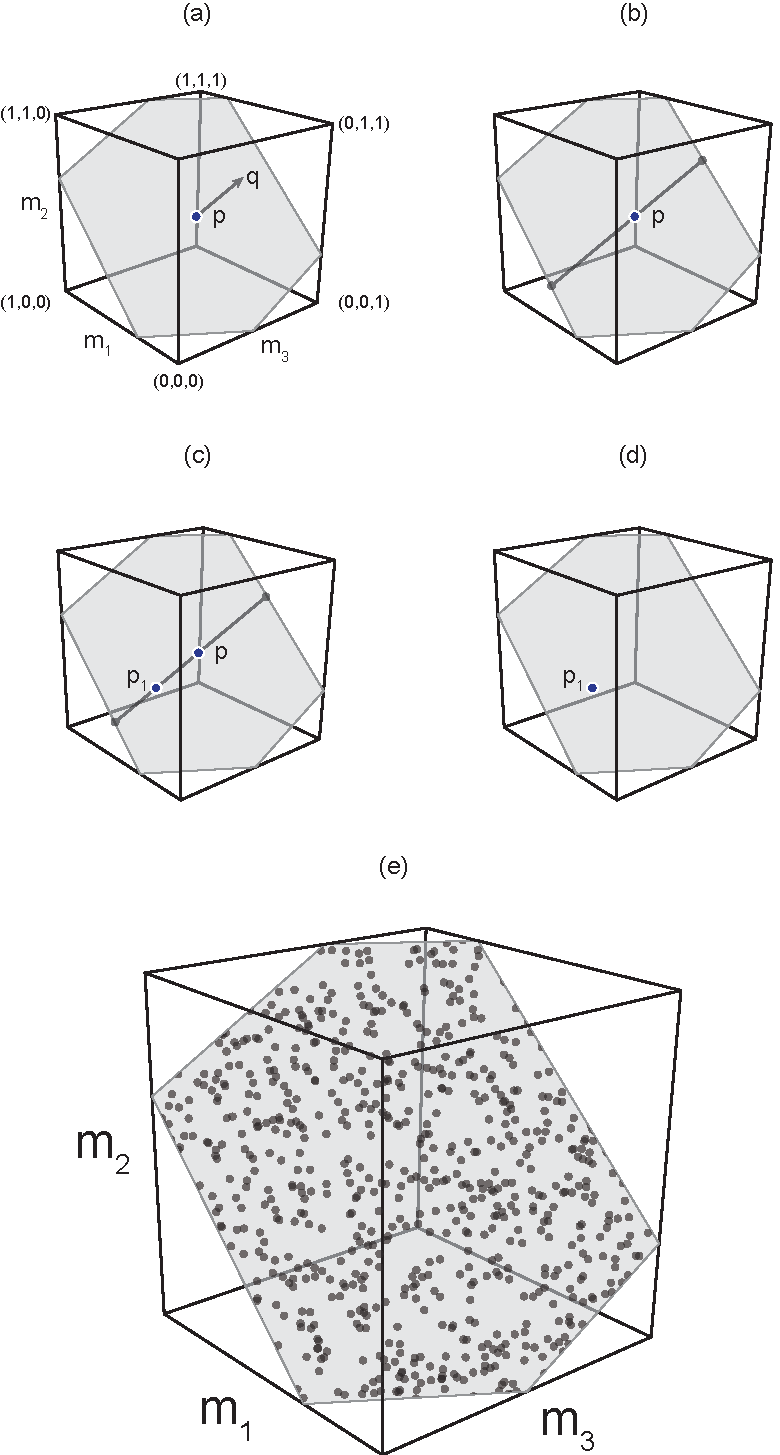
\includegraphics[width=0.5\textwidth]{numbered_figures/figure_2_hit_and_run_ALL_steps.pdf}
\caption{\textbf{Characterizing the high-dimensional structure of a feasible activation set via the Hit-and-Run algorithm~\cite{lovasz1999hit}.}  For a large class of biomechanical tasks, the feasible activation set is a convex polytope. Here we show a 3-muscle system as a schematic example upon which Hit-and-Run can be applied. We select a valid direction at random (a), and project a line to both boundaries (b). After selecting a point at random from the resulting line (c), we get a new valid point $p_1$ (d). Repeating steps a-d many (e.g., 100,000) times, and down-sampling those points, produces a statistically complete representation of the polytope (e)---and of the high-dimensional structure of the feasible activation set.}
\label{fig:figure_2_hit_and_run_steps}
\end{figure}
The Hit-and-Run algorithm is defined as follows (it works analogously for any convex body even if not a polytope)\cite{lovasz1999hit}:
\begin{enumerate}
\item Find a point $\textbf{p}$ in $P$ to use as a starting point by using the linear programming method documented in the Supplementary Note.
\item Generate a line in a random direction $q$ (uniformly-at-random\ over all directions) from $\textbf{p}$ in $P$ (Fig.~\ref{fig:figure_2_hit_and_run_steps}a).
\item Find the two intersection points of the line given by the random direction $q$ with the boundary of the polytope (Fig.~\ref{fig:figure_2_hit_and_run_steps}b).
\item Choose a new point uniformly-at-random on the line segment between the intersection points (Fig.~\ref{fig:figure_2_hit_and_run_steps}c).
\item Repeat the above steps from $2.$ onwards using the new point as the starting point, and generate a new random direction.
Continue this process for $s$ iterations, where $s$ is the mixing number. The mixing number is the number of iterations that are expected to result in a point sampled uniformly at random from the space, with respect to the starting point (and any other point in $P$. Saving just the $s^{th}$ point for many repetitions will result in many uniform-at-random points collected across the feasible activation space (Fig.~\ref{fig:figure_2_hit_and_run_steps}).
\end{enumerate}



Experimentally, it is known to converge to a uniform sampling across any convex body, up to about 40 dimensions~\cite{smith1984efficient}. The Hit-and-Run method is a generalization of a discrete Markov chain---where the goal is to identify multiple points from the feasible activation polytope $P$ uniformly-at-random.

We describe the mathematical basis and details to replicate our implementation in the Supplementary Note, including our application of slack variables to select a valid starting point within the feasible activation space.




\section*{Supplementary Note: Algorithmic Implementaion of Hit-and-Run}
The polytope $P$ is defined by the mechanics of the limb and the constraints of the task as
\[\textbf{f} = A\textbf{a}, \textbf{a} \in [0,1]^n,\]
and to find a starting point $\textbf{p}$ we need only to find one feasible activation vector in the space.
For the Hit-and-Run algorithm to mix faster we do not want the starting point to be close to a vertex of $P$ ~\cite{Lovasz}. Intuitively, this is because we do not want to get stuck in a corner.
We use the following standard trick with slack variables $\epsilon_i$, which in practice often provides a good starting point for sampling algorithms. In essence, we use the slack variables to find a point far away from the boundaries of the $n$-cube.

\begin{equation}\label{eq:LP_r}
\begin{array}{lrcl}
\mbox{maximize} & \sum_{i=1}^n \epsilon_i \\
\mbox{subject to} & \textbf{f} &=& A\textbf{a}\\
 & a_i &\in& [\epsilon_i, 1- \epsilon_i], \hspace{5mm} \forall i \in \{1,\dots,n\} \\
 & \epsilon_i &\geq& 0, \hspace{5mm} \forall i \in \{1,\dots,n\}.
\end{array}
\end{equation}
Thus running a linear program with these reduced ranges of the variables will produce a starting point that is far from the boundaries of $P$, and is not stuck in a corner.



The rest of the implementation of the Hit-and-Run algorithm is straightforward except for the choice of the random direction $q$. How do we sample u.a.r.\ (uniformly-at-random) from all directions in $P$?
Recall that all points in $P$ are by definition valid solutions to a given task.

The direction of $q$ must be in the null space of the task, which is defined as $V = \{ y \in R^n \mid Ay = 0\}$. Hence we need to choose  directions uniformly at random across the vector space $V$.

As shown by Marsaglia this can be done as follows~\cite{Marsaglia}.
\begin{enumerate}
\item
Find an orthonormal basis $b_1, \dots, b_r \in \mathbb{R}^{n}$ of \{$\textbf{q} \in \mathbb{R}^n | A\textbf{q} = 0$\}.
\item
Choose $(\lambda_1, \dots, \lambda_r) \in \mathcal{N}(0,1)^r$ (from the zero-mean unit-variance Gaussian distribution).
\item
$\sum_{i=1}^r \lambda_i b_i$ is a u.a.r.\ direction.
\end{enumerate}

A basis of a vector space $V$ is a minimal set of vectors that generate $V$, and it is orthonormal if the vectors are pairwise orthogonal (perpendicular) and have unit length. Using basic linear algebra one can find a basis for $\{q \in \mathbb{R}^n | A\textbf{q} = 0\}$ and orthogonalize with the well known Gram-Schmidt method. Note that in order to get the desired uniform and random sample the basis needs to be orthonormal. The limb model is defined such that the rows of $A$ are linearly independent and hence $r=n-m$.

\subsection*{Mixing Time}
\label{sec_lengthrun}
While we have rigorous experimental evidence that supports using Hit-and-Run in this setting, we do not have theoretical proof that guarantees our sampling will mix to the uniform distribution. Hit-and-Run is theoretically guaranteed to mix in time $\mathcal{O}(n^3)$ if the polytope is not too "flat", meaning that the ratio between the inscribed circle and enclosing circle is not too small. Such degenerate examples are usually artificially created and we henceforth assume that this does not happen in our system of muscles.
From a given starting point, how many iterations of the Hit-and-Run method are necessary to reach a u.a.r.\ point?
For convex polytopes in $n$ dimensions up to $40$, experimental results suggest that $\mathcal{O}(n)$ steps of the Hit-and-Run algorithm are sufficient.
In particular, the paper~\cite{emiris2013efficient} by Emiris and Fisikopoulos suggests that selecting every $10(n + 1)$ points is sufficient to get a uniform distribution~\cite{emiris2013efficient}, while in Ge et al.'s paper every single point of the Hit-and-Run algorithm is used in the sample~\cite{Ge}. It's worth noting that these results are experimental, not theoretical.


The Hit-and-Run algorithm was specifically developed to address $\#P$-hard problems such as approximating the volume of high-dimensional polytopes\cite{Dyer}. The Hit-and-Run algorithms can converge to the uniform sampling across any convex body~\cite{smith1984efficient} after $\mathcal{O}^*(n^2R^2/r^2)$ steps ($r$ and $R$ are the radii of the inscribed and circumscribed ball of the polytope as mentioned in the Introduction)~\cite{Dyer, Lovasz}. Experimental results suggest that a number of points linear with respect to $N$ suffices for convex polytopes embedded in dimensions up to 40. Emiris and Fisikopoulos~\cite{emiris2013efficient} suggest that $(10 + \frac{10}{N})~N$ iterations suffice to uniformly sample a convex polytope.

\subsection*{Data and code availability}
All analyses are replicable and extensible with Open Source libraries. We developed and tested our code in Ubuntu 14.04, Windows 8.1, and OSX Yosemite 10.12.1; implemented Hit-and-Run with Scala 2.11.6, and developed visualizations with R 3.3.0.
All figure source data are available within the repository https://github.com/briancohn/space.

\section*{Acknowledgments}


\section*{Author contributions and Correspondence}
M.S. derived the mathematics of our Hit-and-Run implementations, B.C. implemented those algorithms and designed the simulations. F.V.C supported the neurobiological interpretations, while B.G. supported work with computational geometry. F.V.C. can be contacted via valero@usc.edu.

\section*{Competing Financial Interests}
We do not have any competing interest to declare.

% \nolinenumbers

\bibliography{plos_cohn_bibliography.bib}
% \bibliographystyle{plain}

\end{document}
